\documentclass{article}
\usepackage[utf8]{inputenc}
\usepackage{geometry}
\geometry{margin=0.75in}

\title{Cache Coherence for Phase-Concurrent Programs}
\author{Anson Kahng, Charles McGuffey, and Sam Westrick}
\date{May 2017}

\usepackage{color} % for todos
\usepackage{fixltx2e} % for subscripts
\usepackage{wasysym} % for frownies
\usepackage{float} % for table position
\usepackage{parskip} % for indentation
\usepackage{graphicx} % for images
\usepackage{tikz} % more images
\usepackage{textcomp}


% table line break packages
\usepackage{array}
\usepackage{makecell}

\renewcommand\theadalign{cb}
\renewcommand\theadfont{\bfseries}
\renewcommand\theadgape{\Gape[4pt]}
\renewcommand\cellgape{\Gape[4pt]}

\usepackage{biblatex}
\usepackage{listings}
\lstset{
 basicstyle=\ttfamily,
 mathescape
}

\usepackage{filecontents}

\begin{filecontents*}{general.bib}
@inproceedings{choi2010denovo,
 title={Denovo: Rethinking hardware for disciplined parallelism},
 author={Choi, Byn and Komuravelli, Rakesh and Sung, Hyojin and Bocchino, Robert and Adve, Sarita and Adve, Vikram},
 booktitle={Proceedings of the Second USENIX Workshop on Hot Topics in Parallelism (HotPar)},
 year={2010}
}

@inproceedings{ros2012complexity,
 title={Complexity-effective multicore coherence},
 author={Ros, Alberto and Kaxiras, Stefanos},
 booktitle={Proceedings of the 21st international conference on Parallel architectures and compilation techniques},
 pages={241--252},
 year={2012},
 organization={ACM}
}

@inproceedings{shun2014phase,
 title={Phase-concurrent hash tables for determinism},
 author={Shun, Julian and Blelloch, Guy E},
 booktitle={Proceedings of the 26th ACM Symposium on Parallelism in Algorithms and Architectures},
 pages={96--107},
 year={2014},
 organization={ACM}
}

@article{blumofe1999scheduling,
  title={Scheduling multithreaded computations by work stealing},
  author={Blumofe, Robert D and Leiserson, Charles E},
  journal={Journal of the ACM (JACM)},
  volume={46},
  number={5},
  pages={720--748},
  year={1999},
  publisher={ACM}
}

\end{filecontents*}

\addbibresource{general.bib}

\begin{document}

\newcommand{\todo}[1]{{\color{red} \textbf{TODO}: {#1}}}

\maketitle

\section{Introduction}\label{sec:intro}

In an effort to simplify the complexity and improve the scalability of cache coherence schemes, some researchers have begun looking at the benefits of restricted forms of parallelism. For example, it could be reasonable to assume that parallel programs are \textit{data-race free} (DRF). Under this restriction, it is possible to obtain improved performance with a simplified protocol \cite{choi2010denovo, ros2012complexity}.

However, while DRF programs are common, there are some programs which benefit from ``well-behaved'' data races. For example, consider the following algorithm, based on the Sieve of Erastosthenes, which generates all primes less than $n$ in parallel.

\begin{lstlisting}
function primes(n) {
  if n < 2 then return {};
  let isPrime = [true : 0 $\leq$ i < n];
  foreach p in primes($\sqrt{n}$) {
    foreach k where 2 $\leq$ k < $\lceil n/p \rceil$ {
      isPrime[p $\cdot$ k] := false;
    }
  }
  return {$i$ : 2 $\leq$ i < n | isPrime[i]};
}
\end{lstlisting}

This algorithm relies on multiple processors writing to the same flag at the same time (write-write races), and is therefore not DRF. However, it does not exhibit read-write races. In this sense its memory locations are phase-concurrent, meaning that they each alternate between concurrent read and concurrent write phases. During a location's read phase, it is read-only. During a write phase, it is write-only. Note that phases are not global: it is possible for a process to be reading from one cell while writing to another without synchronizing in between.

In the example algorithm above, there is an added guarantee that concurrent writes to the same location will always be writing the same value. In general, we will not require this, as will be discussed in more detail later.

The term ``phase-concurrent'' is inspired by Shun and Blelloch's work on concurrent hash tables \cite{shun2014phase}.

\section{Definitions and Semantics}

A \textit{program} consists of $P$ dynamic streams of instructions, where $P$ is the number of processes. An \textit{execution} is an interleaving of those $P$ streams produced by some scheduler, where at each time step, the scheduler lets one stream advance by a single instruction.

Two distinct instructions $A$ and $B$ are \textit{concurrent} if there exist two executions $E_1$ and $E_2$ such that $A \prec B$ in $E_1$ and $B \prec A$ in $E_2$, where the relation $X \prec Y$ means $X$ appears before $Y$ in a specific execution. In other words, if the relative order of $A$ and $B$ is not constant over all executions, then $A$ and $B$ are defined to be concurrent.

We distinguish between three classes of atomic memory operations: read, write, and read-modify-write (such as compare-and-swap, fetch-and-add, etc). We say that a multi-threaded program is \textit{phase-concurrent} if all concurrent operations at the \textit{same} memory location are of the same class. In our implementation, we discretize memory locations at the level of cache lines; we later describe how to extend this framework to the granularity of individual memory locations.

Under this definition, phase-concurrent programs must rely on read-modify-write (RMW) operations to synchronize effectively. For example, here is a phase-concurrent program using two processes to sum an array $a$ of length $2n$ and print the result. Both processes run the same code. The value $p$ is the identifier of the process (in this example, 0 or 1). Assume there is some shared cell $s$ initially set to $2$. We use $r$ to store intermediate results, and the RMW operation sub-and-fetch (which atomically subtracts and fetches the new value) to synchronize.

\begin{lstlisting}
function sum_array(a) {
  // initially s == 2
  r[p] := 0;
  for i where p $\cdot$ n $\leq$ i < (p+1) $\cdot$ n {
    r[p] := r[p] + a[i];
  }
  if (sub-and-fetch(s,1) == 0) {
    // exactly one process will execute this
    printf("%d\n", r[0] + r[1]);
  }
}
\end{lstlisting}

Note that this process is actually DRF; we haven't yet discussed how to handle concurrent writes; we do so below.

\subsection{Concurrent Writes}
When two or more processes concurrently write to the same location, we need to specify what value will be returned at the next read. We propose non-deterministically ``choosing a winner".

Specifically, consider a particular execution and a read operation of interest. Identify the write $w$ which occurred most recently before the read, and let $W$ be the set of all writes that are concurrent with $w$. Partition $W$ into sets $W_p$ containing only the writes issued by process p. For each of these, identify the write $w_p$ which is the last write in $W_p$. The winning write is chosen non-deterministically from $\{w_p : 0 \leq p < P\}$.

The above specification is a bit nasty, but (we claim) actually quite intuitive. For each memory location, at the end of each of its write phases, we non-deterministically choose one written value to be visible in the following read phase. The value which is chosen must be the ``last" write of some process within that phase.

For example, we can modify the array-sum example to print not only the sum of the array, but also the identifier of the process which finished their portion of the array first. To illustrate the requirement that the winning write be the ``last" write of some process, consider the assignment $w$ := 42 below. In both processes, within the same write phase of $w$, that value is overwritten. So it will never be visible.

\begin{lstlisting}
r[p] := 0;
for i where p $\cdot$ n $\leq$ i < (p+1) $\cdot$ n {
  r[p] := r[p] + a[i];
}
w := 42; // this value will never be visible
w := p;
if (sub-and-fetch(s,1) == 0) {
  printf("sum: %d\n", r[0] + r[1]);
  printf("winner: %d\n", w);
}
\end{lstlisting}

% to add: initial cache coherence policy and transition diagram, plus explanations of the optimizations

\section{WSI Cache Coherence}
One of the primary challenges in developing a cache coherence protocol for phase-concurrent programs is managing winners and losers at writes. Some existing techniques can be recycled here. For example, in DeNovo, Choi et al. proposed reusing the shared LLC as a directory, allowing them to track the ``owner" of a modified cache line with no asymptotic space overhead \cite{choi2010denovo}. We will utilize a similar trick. \textbf{From now on, we will refer to the \textit{shared LLC} and the \textit{directory} interchangeably.} Note that this approach requires inclusive caching: every line in an L1 cache must also be in the shared LLC.

At the end of a write phase, we need to commit the winning write back to the directory so that it is visible to other processes. Although we could rely on programmer-directed cache self-invalidations, we would rather not do so. Instead, we will conservatively guess that each synchronization instruction is a barrier which signals the end of a phase.

Our first approach to phase-concurrent cache coherence was predicated on the following axioms. Each writer either ``wins'' or ``loses'' --- as a simplest approach, the first writer wins; the shared LLC acts as a directory, as in DeNovo \cite{choi2010denovo}; the winning writer's data must be flushed at a barrier; and the state can transition due to reads, writes, barriers, and directory interactions. This led to our first cache coherence protocol, which we termed WSI, with three states: \textbf{W}inner, \textbf{S}hared, and \textbf{I}nvalid.

Intuitively, WSI ensures that data can only be in the Shared state during a read phase; during a write phase, data can be in either Winner or Invalid, depending on whether or not the corresponding processor won the write-write race.

For a particular line in an L1 cache, the events which cause state transitions are as follows.

\begin{enumerate}
\item \textbf{(Wr) Write}: a write to this line, issued by the local processor.
\item \textbf{(Re) Read}: a read of this line, issued by the local processor.
\item \textbf{(Ba) Barrier}: a read-modify-write of any line, issued by the local processor.
\item \textbf{(Co) Conflict}: a message from the directory indicating a write to this line by some other processor.
\item \textbf{(Fo) Forward}: a message from the directory indicating a read of this line by some other processor. The cache has to respond to this directory by sending the contents of the line.
\item \textbf{(Ev) Eviction}: an eviction of this line due to the local caching policy.
\end{enumerate}

\begin{table}[H]
\centering
\caption{WSI cache transitions.}
\label{wsi-cache-protocol}
\begin{tabular}{|c|c|c|c|}
\hline
 & \textbf{W} & \textbf{S} & \textbf{I} \\ \hline
\textbf{Wr} & W & W/I & W/I \\ \hline
\textbf{Re} & S & S & S \\ \hline
\textbf{Ba} & I & I & I \\ \hline
\textbf{Co} & W & - & - \\ \hline
\textbf{Fo} & - & S & - \\ \hline
\textbf{Ev} & I & I & I \\ \hline
\end{tabular}
\end{table}

Although WSI is a correct cache coherence policy for phase-concurrent programs, it suffers from many performance issues because it does not take advantage of privacy, does not track ``losers'' in each write phase, and sometimes invalidates data too early to be of use; each of these issues is addressed below.

\textbf{Private data ($W \rightarrow D, C, W$)}:
In this protocol, we must always conservatively ``reset'' (i.e., transition to Invalid) at all barriers. However, if a processor has exclusive access to a memory location, then interacting with the directory and transitioning into Shared or Invalid are inefficient, the intuition being that if no other processor is trying to access the data, there is no need for communication overhead or unnecessary transitions to states that implicitly assume that more than one processor has access to the data. In order to deal with exclusive data, we created two new states, $D$ and $C$, corresponding to Exclusive Dirty and Exclusive Clean, respectively, in which processors have private ownership of the data.

\textbf{Losers ($I \rightarrow L, I$)}:
By the semantics of phase concurrency, if a processor has lost a write-write race in a write phase, then none of its writes can ever be accepted as valid in this phase. However, because the failed writer will be in Invalid, it has to query the directory upon each attempted write to determine whether or not it won the race. This is clearly quite inefficient and led us to create a new state, \textbf{Loser}, from whence all write attempts fail immediately without communication with the directory.

\textbf{Back-to-back read phases ($S \rightarrow S, O$)}:
Because WSI conservatively transitions to Invalid at every barrier, whether the barrier actually represents a phase transition for each cache line, there is potentially additional inefficiency when a barrier interrupts a continuous read phase, whereupon transitioning into Invalid is unnecessary. Therefore, one optimization is the creation of an Old phase, which itself downgrades to Invalid on a barrier, but can get ``renewed'' to Shared if the data is, indeed, read after a barrier.

Together, these optimizations transformed our original WSI protocol to DCWSOLI, where each old state in WSI is ``expanded'' into others as shown in Figure \ref{wsi-to-dcwsoli}.

\begin{figure}[H]
\centering
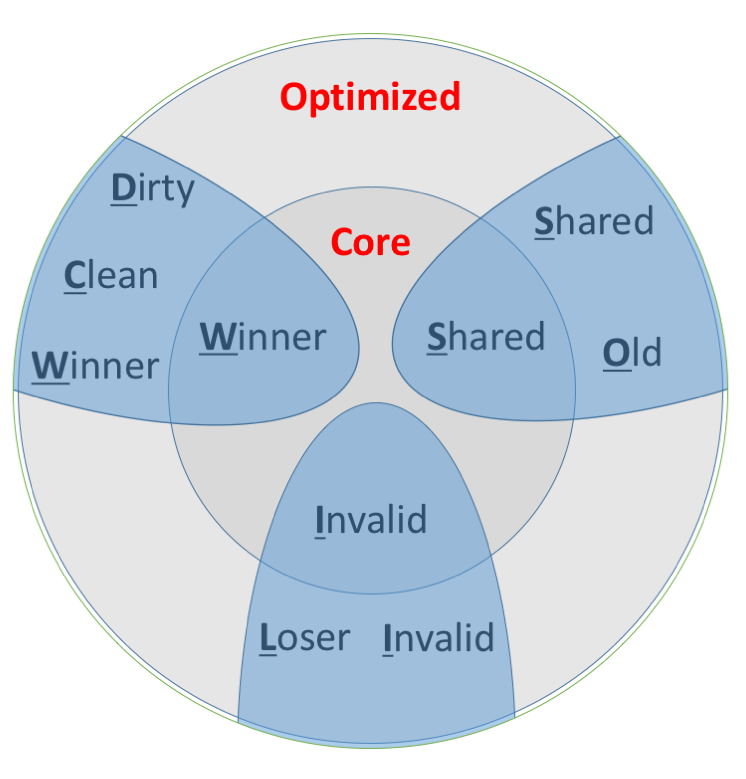
\includegraphics[width=0.4\textwidth]{img/posterfig2.png}
\caption{Basic cache coherence protocol and optimizations.}
\label{wsi-to-dcwsoli}
\end{figure}

\section{DCWSOLI Cache Coherence}
With the above optimizations, the three-state WSI protocol turns into a seven-state protocol we term DCWSOLI (Exclusive \textbf{D}irty, Exclusive \textbf{C}lean, \textbf{W}inner, \textbf{S}hared, \textbf{O}ld, \textbf{L}oser, \textbf{I}nvalid). We now describe the states, transitions, and correctness of this protocol.

\subsection{Local Caches}
Each line in an L1 cache can be in one of seven states. We summarize them briefly here, where we list them from ``most powerful'' to ``least powerful''.

\begin{enumerate}
\item \textbf{(D) Exclusive Dirty:} this is the only valid copy of the line in the system, and it is dirty. No other processors have tried to concurrently write to (or read from) this line.
\item \textbf{(C) Exclusive Clean:} this is the only valid copy of the line in the system, and it is clean. No other processors have tried to concurrently write to (or read from) this line.
\item \textbf{(W) Winner:} this is the only valid copy of the line in the system, and it is dirty. At least one other processor has tried to concurrently write to this line.
\item \textbf{(S) Shared:} this is one of (possibly) many valid copies of the line in the system.
\item \textbf{(O) Old:} this is one of (possibly) many copies of the line in the system, but it may be invalid. Unless the data is refreshed by a read, this line needs to be self-invalidated at the next synchronization.
\item \textbf{(L) Loser:} this line is invalid due to some other processor having concurrently written to this line.
\item \textbf{(I) Invalid:} this line is not in the cache.
\end{enumerate}

\subsection{Directory}
Each line in the directory can be in one of 5 states. The basic idea is to keep track of the status of the owner if possible.

\begin{enumerate}
\item \textbf{(D\textsubscript{p}) Registered $p$ as dirty}: the only valid copy of this line is in state \textbf{D} and is stored in processor $p$'s local cache ($0 \leq p < P$). The local storage reserved for this cache line is overwritten by the identifier $p$.
\item \textbf{(C\textsubscript{p}) Registered $p$ as clean}: the only valid copy of this line is in state \textbf{C} and is stored in processor $p$'s local cache ($0 \leq p < P$). The local storage reserved for this cache line is overwritten by the identifier $p$.
\item \textbf{(W\textsubscript{p}) Registered $p$ as winner}: the only valid copy of this line is in state \textbf{W} and is stored in processor $p$'s local cache ($0 \leq p < P$). The local storage reserved for this cache line is overwritten by the identifier $p$.
\item \textbf{(V) Valid}: this is one of (possibly) many valid copies of the line in the system.
\item \textbf{(I) Invalid}: this line is not in the directory.
\end{enumerate}

For a particular line in the directory, the events which cause state transitions are as follows. They are indexed by the processor identifier of the sender.

\begin{enumerate}
\item \textbf{(Wr\textsubscript{i}) Write}: processor $i$ wants to write to this line. The directory may have to respond to this message with either an accept or reject.
\item \textbf{(Ac\textsubscript{i}) Acquire}: processor $i$ wants to read from this line, and is not currently a sharer of it. The directory has to respond to this message with an accept or reject as well as the contents of the line.
\item \textbf{(Cl\textsubscript{i}) Clean}: processor $i$ is downgrading its status from \textbf{D} to \textbf{C}.
\item \textbf{(Sh\textsubscript{i}) Share}: processor $i$ wants to make its (dirty) copy of this line visible to other processors by downgrading its status from \textbf{W} to \textbf{O}. The processor also has to send the contents of the line.
\item \textbf{(Fl\textsubscript{i}) Flush}: processor $i$ wants to push this line out of its cache. The processor also has to send the contents of the line.
\end{enumerate}

\subsection{Cache Coherence Protocol}
The above states and transition events are coordinated in a message-passing style as follows. Transitions marked - are impossible, and those marked ~\frownie~ violate phase-concurrency.

\begin{table}[H]
\centering
\caption{Transitions for L1 cache $i$. All messages are sent to (and received from) the directory only. For transitions written $A/B$, we transition to $A$ if the directory replies with an accept and $B$ if it rejects.}
\label{cache-protocol}
\begin{tabular}{|c|c|c|c|c|c|c|c|}
\hline
 & \textbf{D} & \textbf{C} & \textbf{W} & \textbf{S} & \textbf{O} & \textbf{L} & \textbf{I} \\ \hline
\textbf{Wr} & D & \makecell{Send Wr\textsubscript{i};\\ D} & W & \makecell{Send Wr\textsubscript{i};\\ D/L} & \makecell{Send Wr\textsubscript{i};\\ D/L} & L & \makecell{Send Wr\textsubscript{i};\\ D/L} \\ \hline
\textbf{Re} & D & C & \frownie & S & S & \makecell{Send Ac\textsubscript{i};\\ Receive data;\\ C/S} & \makecell{Send Ac\textsubscript{i};\\ Receive data;\\ C/S} \\ \hline
\textbf{Ba} & \makecell{Send Cl\textsubscript{i};\\ C} & C & \makecell{Send Sh\textsubscript{i};\\ Send data;\\ O} & O & I & I & I \\ \hline
\textbf{Co} & W & I & - & - & - & - & - \\ \hline
\textbf{Fo} & - & \makecell{Send data;\\ S} & - & - & - & - & - \\ \hline
\textbf{Ev} & \makecell{Send Fl\textsubscript{i};\\ Send data;\\ I} & \makecell{Send Fl\textsubscript{i};\\ Send data;\\ I} & \makecell{Send Fl\textsubscript{i};\\ Send data;\\ I} & I & I & I & - \\ \hline
\end{tabular}
\end{table}

\begin{table}[H]
\centering
\caption{Transitions for the directory.}
\label{directory-protocol}
\begin{tabular}{|c|c|c|c|c|c|}
\hline
 & \textbf{D\textsubscript{p}} & \textbf{C\textsubscript{p}} & \textbf{W\textsubscript{p}} & \textbf{V} & \textbf{I} \\ \hline
\textbf{Wr\textsubscript{i}} & \makecell{Assert $i \neq p$; \\ Reject $i$; \\ Send Co to $p$; \\ W\textsubscript{p}} & \makecell{if $i = p$ then D\textsubscript{p}; \\ else: \{ Accept $i$; \\ Send Co to $p$; \\ W\textsubscript{i}\}} & \makecell{Assert $i \neq p$; \\ Reject $i$; \\ W\textsubscript{p}} & \makecell{Accept $i$; \\ D\textsubscript{i}} & \makecell{Accept $i$; \\ D\textsubscript{i}} \\ \hline
\textbf{Ac\textsubscript{i}} & \frownie & \makecell{Send Fo to $p$; \\ Receive data from $p$; \\ Reject $i$; \\ Send data to $i$; \\ V} & \frownie & \makecell{Reject $i$; \\ Send data to $i$; \\ V} & \makecell{Retrieve data; \\ Accept $i$; \\ Send data to $i$; \\ C\textsubscript{i}} \\ \hline
\textbf{Cl\textsubscript{i}} & \makecell{Assert $i = p$; \\ C\textsubscript{p}} & - & - & - & - \\ \hline
\textbf{Sh\textsubscript{i}} & - & - & \makecell{Assert $i = p$; \\ Receive data from $p$; \\ V} & - & - \\ \hline
\textbf{Fl\textsubscript{i}} & \makecell{Assert $i = p$; \\ Receive data from $p$; \\ V} & \makecell{Assert $i = p$; \\ Receive data from $p$; \\ V} & \makecell{Assert $i = p$; \\ Receive data from $p$; \\ V} & - & - \\ \hline

\end{tabular}
\end{table}

Note that there are only five directory states, so there will be no asymptotic space overhead, as these states can be encapsulated in a constant number of specially treated bits (in this case, 3).

Some of the more interesting transitions in the L1 cache are discussed below.
\begin{itemize}
  \item Receiving a \textbf{Co} while in \textbf{D}: this occurs when another
  process issues a write after the current process successfully wrote to the line. In this scenario,
  the current process becomes the winner and the other process becomes a loser. This is one of the
  core mechanics of the protocol. It describes the mechanics of both losing
  exclusivity and managing winners for phase-concurrency.
  \item Transitioning from \textbf{W} to \textbf{O} at a barrier: note that it
  is also correct to transition to \textbf{C} instead of \textbf{O}. However,
  we predict that in the general case, a line which had conflicting accesses in
  the past will likely have concurrent reads in the futures. Transitioning
  to \textbf{O} reduces the latency of accesses by other processes through keeping the information at the directory rather than the last L1 cache.
  \item Notifications for \textbf{D \textrightarrow{} C} and
  \textbf{C \textrightarrow{} D} transitions: notice that even for private data,
  the L1 caches send messages (\textbf{Wr\textsubscript{i}} and \textbf{Cl\textsubscript{i}})
  to the directory at writes and reads. This is to
  make sure the directory is always informed of the current state of the owner,
  which simplifies its logic and allows the directory to more efficiently transition upon contention. The performance penalty is small, because there
  will be at most 2 messages sent per barrier (the design of parallel
  algorithms typically aims to eliminate synchronization as much as possible,
  so barriers should be infrequent).
  \item Issuing writes while in \textbf{S}: it might at first seem in violation
  of phase-concurrency for a write to be issued while in \textbf{S}, since we
  arrive in \textbf{S} due to concurrent reads and therefore must be in a
  read phase. However, this is incorrect. The directory does not always
  know of exclusivity, and may need to send a process to \textbf{S} conservatively
  at an \textbf{Ac\textsubscript{i}} message even when it would be correct to
  send them to \textbf{C}. For this reason, writes are permitted while in
  \textbf{S}, and the same logic as for \textbf{O} is used.
\end{itemize}

\section{Simulations}

Using a homegrown simulator, we have verified the correctness of the DCWSOLI
protocol on two sample programs, summarized below. Our simulator implements
DCWSOLI assuming that all transitions are atomic (in practice, there would
likely be many transient states in the protocol to handle race conditions).
On both programs, we ran the simulator with many different input sizes and a
a varying number of processors.
\begin{itemize}
  \item \texttt{primes}: as in the example given in Section~\ref{sec:intro},
  this program calculates all primes below a given number in parallel via the
  Sieve of Eratosthenes.
  \item \texttt{hashing}: this program constructs a hash set containing the
  elements of $[n]$ by, on each round, attempting to insert all remaining
  keys and retrying on the next round for those that do not succeed (due to
  losing a write-race). We use open addressing with linear probing.
\end{itemize}
Of course, these programs alone are not representative enough to prove that
our protocol is correct in general. For example, both programs are statically
scheduled in a BSP style. However, one could imagine writing a phase-concurrent
work-stealing scheduler (\cite{blumofe1999scheduling}) in order to support
dynamically scheduled, structured parallel computations.

Unfortunately, due to various technical difficulties, we were unable to conduct
an empirical evaluation comparing our performance against state-of-the-art
protocols such as MESI/MOESI.

% \section{Discussion}
% \todo{Fill in here}

\section{Future Extensions}
\textbf{Sub-cacheline granularity}: As mentioned previously, our current scheme interprets memory at the granularity of cache lines. It is possible to extend this scheme to sub-cacheline granularity, in a way similar to that of DeNovo, at a potentially linear factor of memory overhead in the size of each cache line \cite{choi2010denovo}. Intuitively, supporting sub-cacheline granularity involves replicating each cache line and keeping track of part of each copy of the line. To be precise, if there are $k$ memory locations in cache line $L$, create lines $L_1, \dots, L_k$ and for line $L_i$, classify the entire line solely based on the state of memory location $i$. This therefore requires an extra $\log k$ bits for bookkeeping on each of $k-1$ new copies of each cache line, resulting in $k \log k$ times as much space per original cache line.

\textbf{Larger hierarchies}: So far, we only deal with private L1 and shared L2 caches; one potential future direction of this work is to extend the framework to accomodate larger cache hierarchies, as illustrated by Figure \ref{multi-hierarchy}. Intuitively, this could be done by, for example, recursively viewing all higher-level caches as directories for their children. In particular, each higher-level cache would view the lower-level caches above it as a black-boxed version of the L1 cache in our current protocol. However, we would have to implement extended directory interactions; directories must be able to receive messages from lower- and higher-level directories in order to implement our coherence policy in this recursive manner.

\begin{figure}[H]
\begin{center}
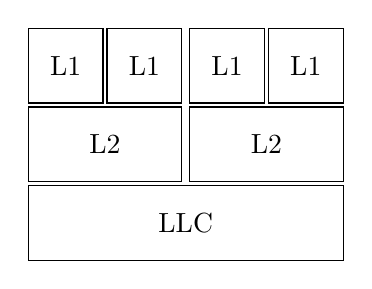
\begin{tikzpicture}
\draw (0,0) rectangle (4, 0.95) node[pos=.5] {LLC};
\draw (0,1) rectangle (1.95,1.95) node[pos=.5] {L2};
\draw (2.05,1) rectangle (4,1.95) node[pos=.5] {L2};
\draw (0,2) rectangle (0.95,2.95) node[pos=.5] {L1};
\draw (1,2) rectangle (1.95,2.95) node[pos=.5] {L1};
\draw (2.05,2) rectangle (3,2.95) node[pos=.5] {L1};
\draw (3.05, 2) rectangle (4,2.95) node[pos=.5] {L1};
\end{tikzpicture}
\end{center}
\caption{Higher-level cache hierarchy.}
\label{multi-hierarchy}
\end{figure}

\textbf{Barrier coalescing}: Another further optimization is \textit{barrier coalescing}, where two or more consecutive barriers at a memory location are grouped together and treated as two ``effective'' barriers. This is potentially useful in the case where there are no intervening memory accesses of the cache line \textit{from the processor's point of view} between many consecutive barriers, and therefore repeatedly downgrading at barriers may be an unnecessary and inefficient policy. However, note that we cannot treat many consecutive barriers as a single barrier because of our transitions from $S$ to $O$ and then $O$ to $I$ on barriers; if we try to coalesce too many barriers with no intervening activity \textit{for a single processor} into one, then we may keep data that has been invalidated by writes by other processors (i.e., to ensure correctness, we need to transition to $I$ instead of $O$).

\printbibliography


\end{document}
